\chapter{Evaluation}
\label{sec:eval}

Our evaluation answers the following questions:

\begin{itemize}
%\begin{itemize}[leftmargin=*]
    \item What is the performance of \prism in terms of transaction throughput and confirmation latency, and how does it compare with other protocols? (\S\ref{sec:eval-performance})
    \item How well does \prism scale to larger numbers of users? (\S\ref{sec:eval-scale})
    \item How does \prism perform with limited resource, and how efficient does it utilize resource? (\S\ref{sec:eval-resource})
    %\todo{``What's the overhead of \prism in terms of CPU and network bandwidth''}
    \item How does \prism perform when under attack? (\S\ref{sec:eval-attack})
\end{itemize}

%\smallskip

\noindent{\bf Schemes compared:} We compare \prism with \algorand, \bng, and the longest chain protocol. For \bng and the longest chain protocol, we modify and use our \prism codebase to enable a fair comparison of the protocols. For \algorand, we use the official open-source implementation~\cite{algorandcode} written in Golang. Note that this implementation is different from the one evaluated in~\cite{algorand}. Therefore, we do not expect to reproduce the results in~\cite{algorand}.

\noindent{\bf Testbed:} We deploy our \prism implementation on Amazon EC2's \texttt{c5d.4xlarge} instances with 16 CPU cores, 16 GB of RAM, 400 GB of NVMe SSD, and a 10 Gbps network interface. Each instance hosts one \prism client. By default, we use 100 instances and connect them into a random 4-regular graph topology. To emulate a wide-area network, we introduce a propagation delay of 120~ms on each link to match the typical delay between two distant cities~\cite{pingmeasurement}, and a rate limiter of 400~Mbps for ingress and egress traffic respectively on each instance. We also evaluate several other network topologies (with up 1000 instances) and per-instance bandwidth limits.

To generate workloads for those experiments, we add a transaction generator in our testbed which continuously creates transactions at an adjustable rate. In our \prism implementation, the main bottleneck is RocksDB and the I/O performance of the underlying SSD, which limits the throughput to about $80,000$ tps. 
We cap transaction generation rate to 75,000 tps to avoid hitting this bottleneck.

%\ly{The \algorand implementation can support at most $4,800$ tps according to our test on the same hardware. As shown later in this section, we are not bottlenecked by it. As a result, the comparison with \algorand is fair.}

%\smallskip
\noindent{\bf Performance tuning and security:} All protocols in the experiments have design parameters, and we tried our best to tune these parameters for performance and security. For \prism, we calculate the optimal mining rate $f$ for proposer and voter blocks to achieve the best confirmation latency, given the adversarial ratio $\beta$ and desired confirmation confidence $\epsilon$. We cap the size of transaction blocks to be 40 KB, and set the mining rate for transaction blocks such that they support $80,000$ tps. Unless otherwise stated, we turn off the spam mitigation mechanism in \prism (we evaluate its effectiveness in \S\ref{sec:eval-attack}).  To ensure security, we calculate the expected {\em forking rate} $\alpha$, i.e. fraction of blocks not on the main chain, given $f$ and the block propagation delay $\Delta$. We compare $\alpha$ against the forking rate actually measured in each experiment, to ensure that the system has met the target security level. We follow the same process for \bng and the longest chain protocol. For \algorand, we adopt the default security parameters set in its production implementation. Then we hand-tune its latency parameters $\lambda$ and $\Lambda$. Specifically, we reduce $\lambda$ and $\Lambda$ until a round times out, and use the settings that yield the best confirmation latency. For \prism, we target a confirmation confidence, $\epsilon$, in the order of $10^{-9}$. For \bng and the longest chain protocol, we target $\epsilon$ in the order of $10^{-5}$. For \algorand, the blockchain halts with a probability in the order of $10^{-9}$.

\section{Throughput and Latency}
\label{sec:eval-performance}

In this experiment, we measure the transaction throughput and confirmation latency of \prism at different adversarial ratio $\beta$, and compare that with \algorand, \bng and the longest chain protocol. For \algorand, we use its default setting of security parameters, which targets $\beta=20\%$.\footnote{The maximum possible security level for Algorand is $\beta = 33\%$, but its latency is expected to increase substantially as $\beta$ approaches 33\%~\cite{algorand}.} For \bng and the longest chain protocol, we experiment with two adversarial ratios: $\beta=20\%$ and $\beta=33\%$. In both \algorand and the longest chain protocol, there is tradeoff between throughput and confirmation latency by choosing different block sizes. We explore this tradeoff and present it in a curve. For \algorand, we try block sizes between 300 KB to 32 MB. For the longest chain protocol, we try block sizes between 1.7 KB  to  33.6 MB. The parameters used in this experiment are available in Appendix~\ref{apx:datapoints}. All four protocols are deployed on the same hardware and network topology as described above. We run each experiment for a minimum of 10 minutes and report the average transaction throughput and latency. The results are shown in Figure~\ref{fig:compare}.


\noindent{\bf Throughput:}
As shown in Fig. \ref{fig:compare}, \prism is able to maintain the same transaction throughput of around $75,000$ tps regardless of the $\beta$ chosen.
This is because \prism decouples throughput from security by using transaction blocks. In this way, \prism is able to maintain the mining rate for transaction blocks to sustain a constant throughput, while changing the mining rate for other types of blocks to achieve the desired $\beta$. \bng offers a similar decoupling by entitling the miner of the latest key block to frequently produce micro blocks containing transactions. \algorand and the longest chain protocol do not offer such decoupling, so one must increase the block size in order to achieve a higher throughput. In such case, the confirmation latency increases, as demonstrated by the tradeoff curves in Figure~\ref{fig:compare}, to accommodate for the higher block propagation delay induced by larger blocks. For the longest chain protocol, its throughput limit has been discussed in \S\ref{s:lc-thput}.
For \algorand, we observe its throughput increases marginally with block size, but does not exceed $1300$ tps.
The reason is that \algorand only commits one block every round. So at any moment, unlike \prism, \algorand only has one block propagating in the network, causing low bandwidth utilization. For \bng, we observed a peak throughput of 21,530 tps. The reason is that, unlike \prism, in \bng only a single node (the leader) commits transactions at a time. This results in the network becoming a bottleneck; once throughput exceeds about 20,000 tps, we observed that the block propagation delay increases significantly for \bng.\footnote{Note also that Bitcoin-NG is susceptible to an adaptive attack that censors the chosen leader and can reduce throughput substantially~\cite{parallel}.}


\noindent{\bf Is Consensus the Throughput Bottleneck?}
A blockchain client has two roles: (1) it participates in the consensus protocol (the \textit{Block Structure Manager} and the \textit{Miner} in our implementation); (2) it executes transactions confirmed by the consensus protocol and updates the ledger (the \textit{Ledger Manager} in our implementation). The throughput can be bottlenecked by either of these stages and therefore we ask: Is the throughput limited by the consensus protocol, or the ledger updates? To answer this question, we measure the maximal throughput when no consensus protocol is involved, i.e. we start one client of each protocol and test how fast each client can execute transactions and update the ledger. For our \prism, \bng and longest chain client, the limit is around $80,000$ tps. For \algorand, the limit is around $4,800$ tps. From Fig.~\ref{fig:compare} we see that \bitcoin, \bng, and \algorand have throughput much lower than these limits, and thus are bottlenecked by the consensus protocols. However, in case of \prism, its throughput is very close to the limit, and hence it is bottlenecked by the ledger updates.

\noindent{\bf Confirmation Latency:} The confirmation latency of \prism stays below one minute for $\beta \leq 40\%$. At $\beta = 20\%$, \prism achieves a latency of $13$ seconds, and for  similar security guarantees \algorand achieves latency of $2$ seconds. Compared to the longest chain protocol, \prism uses multiple voter chains in parallel ($1000$ chains in our experiments) to provide security instead of relying on a single chain. So \prism requires each vote to be less deep in order to provide the same security guarantee. As a result, \prism achieves a substantially lower confirmation latency. For example, for $\beta = 33\%$, the confirmation latency for \prism is 23 seconds, compared to 639 seconds at the lowest throughput point for the longest chain protocol. As we increase the block size for the longest chain protocol, its  confirmation latency increases to 1956 seconds at a throughput of 282 tps. The gap between \prism and the longest chain protocol increases for higher $\beta$. For example, for \prism the confirmation latency increases from 13 seconds to 23 seconds as $\beta$ increases from $20\%$ to $33\%$. For the longest chain protocol, the same change in $\beta$ causes the latency to increase by more than 800 seconds. \bng exhibits similar confirmation latency as the longest chain protocol for the same value of $\beta$, since it applies the same $k$-deep rule as the longest chain protocol for key blocks to confirm transactions, and key blocks must be mined slowly to avoid frequent leader changes.

%that is $10\times$ better than the longest chain protocol even at its lowest .

\section{Scalability}

\label{sec:eval-scale}
\begin{table}[ht]
	\centering
	\caption{\small Performance of \prism with different network topologies.}
	\begin{tabular}{| c || c | c c c |} 
	 \hline
	 Property & \#Nodes & 100 & 300 & 1000 \\ [0.5ex] 
	 \hline\hline
	 \multirow{4}{*}{Degree $=4$}   & Diameter & 5 & 7 & 9 \\
	                                & Throughput (tps) & $7.2\times 10^4$ & $7.4\times 10^4$ & $7.4\times 10^4$ \\
	                                & Latency (s) & 40 & 58 & 67 \\
	                                & Forking & 0.119 & 0.117 & 0.112 \\
	 \hline
	 \multirow{4}{*}{Diameter $=5$} & Degree & 4 & 6 & 8 \\
	                                & Throughput (tps) & $7.2\times 10^4$ & $7.9\times 10^4$ & $7.9\times 10^4$ \\ 
	                                & Latency (s) &40 & 44 & 37 \\
	                                & Forking & 0.119 & 0.119 & 0.127 \\
	 \hline
	\end{tabular}
	\label{table:scale}
	\end{table}

In this experiment, we evaluate \prism's ability to scale to a large number of users. For each client, we use the same network and hardware configuration as in other experiments, and target an adversarial ratio $\beta=40\%$. The results are shown in Table~\ref{table:scale}.

First, we increase the number of clients while keeping the topology a random 4-regular graph, i.e., each client always connects to four random peers. In this case, the network diameter grows as the topology becomes larger, causing the block propagation delay to increase and the confirmation latency to increase correspondingly. Note that the transaction throughput is not affected\footnote{In the results, the throughput increases as we increase the network size. This is because of an artifact in our testbed which causes slightly more transactions to be generated when there are more nodes in the network.} because in \prism the mining rate for transaction blocks is decoupled from that of the other types of blocks. Then, we explore the case where clients connect to more peers as the topology grows larger, so that the diameter of the network stays the same. As shown in the results, both confirmation latency and throughput are constant as the number of clients increases from 100 to 1000. 

In all cases, the forking rate stays stable and is under $0.13$, proving that the system is secure for $\beta=40\%$. This suggests that \prism is able to scale to a large number of users, as long as the underlying peer-to-peer network provides a reasonable block propagation delay. We also provide the distributions of block propagation delay in each topology in Appendix~\ref{apx:propagation}.

\section{Resource Utilization}
\label{sec:eval-resource}

In this experiment, we evaluate the resource utilization of our \prism implementation, and how it performs with limited network bandwidth and CPU resources. 

% resources. Generally \prism uses the following three resources: CPU, to verify cryptographic signatures, to execute transactions, and to assemble blocks. Storage, to store the ledger and blocks. Network, to receive and broadcast blocks from/to peers.




\begin{figure}
    \centering
    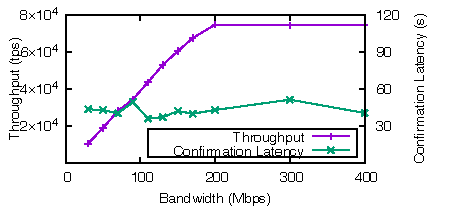
\includegraphics[width=0.75\textwidth]{figures/resource-fig-bw.pdf}
    \caption{\small Performance of \prism with different network bandwidth at each client. The in-memory size of a transaction is 168 bytes.}
    \label{fig:bw}
\end{figure}

\begin{table}[ht]
\centering
\caption{\small Network bandwidth usage breakdown of \prism measured on a 200 Mbps interface. Network Headroom is the unused bandwidth necessary for the block propagation delay to stay stable. Serialization overhead is wasted space when serializing in-memory objects for network transmission. Messaging stands for non-block messages.}
\begin{tabular}{| c | c | c || r |} 
 \hline
 \multicolumn{3}{|c||}{Usage} & $\%$Bandwidth \\ [0.5ex] 
 \hline\hline
 \multirow{5}{*}{Received} & \multirow{4}{*}{Deserialized} & Proposer Block & $0.05\%$ \\
 && Voter Block & $0.21\%$ \\
 && Transaction Block & $50.43\%$ \\ \cline{3-4}
 && Messaging &  $0.43\%$ \\ \cline{2-4} 
 & \multicolumn{2}{|c||}{Serialization Overhead} & $25.80\%$ \\ \hline
 \multicolumn{3}{|c||}{Network Headroom} & $23.08\%$ \\
 \hline
\end{tabular}

\label{table:bw-profiling}
\end{table}

\noindent{\bf Network Bandwidth:} Figure~\ref{fig:bw} shows the throughput and confirmation latency of \prism as we throttle the bandwidth at each client. Results show that the confirmation latency is stable, and the throughput scales proportionally to the available bandwidth. The throughput stops to grow when the bandwidth is higher than 200 Mbps, because the transaction generation rate is capped at 75,000 tps, which is near the bottleneck caused by RocksDB.

Table~\ref{table:bw-profiling} provides a breakdown of bandwidth usage. Our implementation is able to process transaction data at a throughput about $50\%$ of the available bandwidth. Further improvements could be made by using more efficient data serialization schemes and optimizing the underlying P2P network.

\begin{figure}
    \centering
    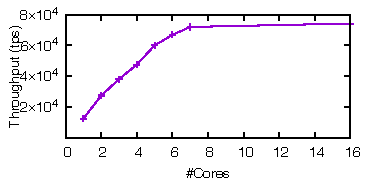
\includegraphics[width=0.65\textwidth]{figures/resource-fig-cpu.pdf}
\caption{\small Performance of \prism with different number of CPU cores at each client}
    \label{fig:cpu}
\end{figure}

\noindent{\bf CPU:} Figure~\ref{fig:cpu} shows the throughput of \prism as we change the number of CPU cores for each client. The throughput scales proportionally to the number of cores, and stops to grow after 7 cores because the transaction generation rate is capped. This shows that our implementation handles more than 10,000 tps per CPU core, and the parallelization techniques discussed in \S\ref{sec:implementation} are effective. 

Table~\ref{table:profiling} provides a breakdown of CPU usage across different components. More than half of CPU cycles are taken by RocksDB for which we only perform basic tuning. Less than $15\%$ are spent on overhead operations, such as inter-thread communication, synchronization, etc. (categorized as ``Miscellaneous'' in the table). This suggests that our implementation uses CPU resources efficiently, and further improvements could be made primarily by optimizing the database. 

While we chose mid-end AWS EC2 instances for  experiments, our results show that  \prism  does not inherently require powerful machines or waste resources.\footnote{For example, a laptop with 8 cores, 16 GB RAM, and 400 GB of NVMe-based SSD would cost under \$3,000 today and could easily run Prism.} On the contrary, its high resource efficiency and scalability that we demonstrate in this experiment makes \prism suitable for applications with different requirements. 

%This suggests that our implementation design mentioned in Section~\ref{sec:implementation-highlights} enables efficient and scalable parallelization.

\begin{table}[ht]
\centering
\caption{\small CPU usage breakdown of our \prism implementation.}
\begin{tabular}{| c | c || r |} 
 \hline
 \multicolumn{2}{|c||}{Operation} & $\%$CPU \\ [0.5ex] 
 \hline\hline
 %\multirow{5}{*}{Ledger} & RocksDB Read & $13.2\%$ \\ %\cline{2-3}
 %                        & RocksDB Write & $13.1\%$ \\ %\cline{2-3}
 \multirow{3}{*}{Ledger} & RocksDB Read/Write & $49.5\%$ \\ %\cline{2-3}
                         & (De)serialization & $3.1\%$\\ %\cline{2-3}
    %                     & Serialization & $2.0\%$\\ %\cline{2-3}
    %                     & Deserialization & $1.1\%$ \\ %\cline{2-3}
                         & Miscellaneous & $8.9\%$\\ \hline
 \multirow{5}{*}{Blockchain}    & Signature Check & $21.7\%$ \\ %\cline{2-3}
                         & (De)serialization & $3.8\%$ \\
                         & RocksDB Read/Write & $3.9\%$ \\
 %                        & Serialization & $2.0\%$\\ %\cline{2-3}
 %                        & Deserialization & $1.8\%$ \\ %\cline{2-3}
                         & Network I/O & $0.6\%$ \\ %\cline{2-3}
                         & Miscellaneous & $5.5\%$\\ \hline
% \multicolumn{2}{|c||}{RocksDB Background Jobs} & $25.0\%$ \\ \hline
  \multicolumn{2}{|c||}{Block Assembly} & $1.5\%$ \\ \hline
 \multicolumn{2}{|c||}{Transaction Generation} & $0.7\%$ \\ \hline
 \multicolumn{2}{|c||}{Miscellaneous} & $0.8\%$ \\ \hline
\end{tabular}
\label{table:profiling}
\end{table}

\section{Performance Under Active Attack}
\label{sec:eval-attack}

In the following experiments, we evaluate how \prism performs in the presence of active attacks. Specifically, we consider three  types of attacks: {\em spamming}, \textit{censorship}, and \textit{balancing} attacks. Spamming and censorship attacks aim to reduce network throughput, while balancing attacks aim to increase confirmation latency. 
%For censorship and balancing attacks, we configure a variable fraction of clients to be malicious and measure the throughput and latency of the system. 
In these experiments we configure \prism to tolerate a maximum adversarial ratio $\beta=40\%$. 

%We will demonstrate that the performance of \prism degrades gracefully under active attacks.
%\todo{cite https://eprint.iacr.org/2016/555.pdf}



\label{sec:spamming-eval}
\noindent{\bf Spamming Attack.} Recall that in a spamming attack, attackers send conflicting transactions to different nodes across the network. As described in \S\ref{sec:spamming-design}, miners can mitigate such attack by adding a random timing jitter to each transaction. In this experiment, we set up 100 miners as victims and connect them according to the same topology as in other experiments. Then for each miner we start a local process that generates a transaction every 100 ms. We synchronize those processes across the network so that each miner receives the same transaction at the same time, with a time synchronization error of several ms due to the Network Time Protocol. 
To defend against the attack, miners add a uniform random delay before including a transaction into the next transaction block. We let each attack to last for 50 seconds, and measure the fraction of spam transactions that end up in transaction blocks. 
Fig.~\ref{fig:attack-spamming} shows that adding a random jitter of at most 5 seconds can reduce the spam traffic by about 80\%. 
We point out that miners can extend this method by monitoring the reputation of clients by IP address and public key, and penalizing clients with high spam rate with longer jitter.

%\gf{Notice that the protocols we compare against (the Longest Chain protocol, Algorand, Bitcoin-NG) are not susceptible to these attacks because transactions are validated prior to block creation.}
%An adversary could generate a large number of conflicting transactions and disseminate them to different nodes across the network.  
%The 
%spam/duplicate transactions
% There are a few practical mechanisms for circumventing this. 
%To circumvent this, nodes should first validate transactions with respect to their latest ledger state and other unreferred transaction blocks, 
%\gw{I think ledger state is more proper than ledger tip.}
%giving the adversary only a small window of network delay to spam the system. % and thus significantly weakens the attack.
%Second, miners could add some timing jitter prior to mining transactions, 
%giving other miners the ability to observe if a conflicting transaction is already present in a transaction block, in  which case the miner will choose to not include that transaction. % in its block.
%We evaluate the effectiveness of this method in \S\ref{sec:spamming-eval}.

\if 0
\noindent{\bf Spamming Attack.} In Prism, miners do not validate transactions before including them in blocks. 
% This raises practical issues, namely spam. 
This introduces possible spamming attacks, where attackers send conflicting transactions to different nodes across the network. 
Nodes would then mine all of these transactions into blocks, causing miners and validators to waste storage and computational  resources.

\ly{
To circumvent this issue with Prism, we propose validating transactions with respect to their latest ledger state and other unconfirmed transactions, giving the adversary only a small window of network delay to spam the system. 
Miners can then mitigate spamming attacks by adding a random timing jitter prior to mining transactions, giving other miners the ability to observe if a conflicting transaction is already present in a transaction block, in  which case the miner will choose to not include that transaction. In this experiment, we set up 100 miners as victims and connect them according to the same topology as in other experiments. Then for each miner we start a local process that generates a transaction every 100 ms. We synchronize those processes across the network so that each miner receives the same transaction at the same time, with a time synchronization error of several ms due to the Network Time Protocol. 
To defend against the attack, miners add a uniform random delay before including a transaction into the next transaction block. We let each attack last for 50 seconds, and measure the number of transactions that end up in transaction blocks. The higher the number is, the more spam traffic the attacker has been able to create.
Fig.~\ref{fig:attack-spamming} shows that adding a random jitter of at most 5 seconds can reduce the spam traffic by about 80\%. 
We point out that miners can extend this method by monitoring the reputation of clients by IP address and public key, and penalizing clients with high spam rate with longer jitter.
} 
\gw{We also present an analysis to show that another distribution of random jitter, namely, exponential distribution is also helpful to mitigate spam attacks in Appendix~\ref{app-spam}.}

\fi

\begin{figure}
    \centering
    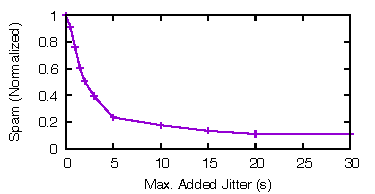
\includegraphics[width=0.65\textwidth]{figures/attack-fig-spamming.pdf}
    \caption{\small Effectiveness of random jitter in defending against spam attack. Jitters follow uniform distributions and we report the maximum jitter that we add. Spam traffic amount is normalized to the case when no jitter is added.}
    \label{fig:attack-spamming}
\end{figure}









\begin{figure}
    \centering
    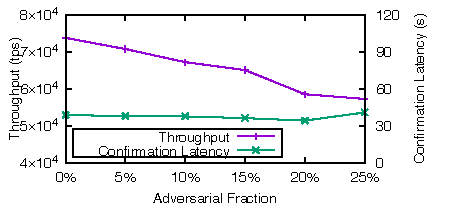
\includegraphics[width=0.75\textwidth]{figures/attack-fig-censor.pdf}
    \caption{\small Performance of \prism under  censorship attack.}
    \label{fig:attack-censor}
\end{figure}

\noindent{\bf Censorship Attack.}
In a censorship attack, malicious clients mine and broadcast empty transaction blocks and proposer blocks. Censorship attack does not threaten the security of \prism, but it reduces the system throughput because a portion of blocks are now ``useless'' since they do not contain any data. As Figure~\ref{fig:attack-censor} shows, during a censorship attack, the transaction throughput reduces proportionally to the percentage of adversarial users. Theoretically, censorship attack could also affect the confirmation latency, because it could take longer for a transaction block to be referred to if some proposer blocks are empty. However, since a proposer block is mined roughly every 10 seconds, the impact on latency is nominal. Our results shows that the confirmation latency stays stable as we increase the adversarial ratio from $0\%$ to $25\%$.


\label{sec:balancing}

\begin{figure}
    \centering
    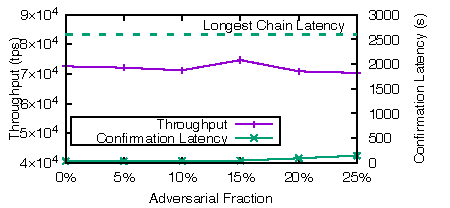
\includegraphics[width=0.75\textwidth]{figures/attack-fig-balancing.pdf}
    \caption{\small Performance of \prism under balancing attack. We also mark the confirmation latency of the longest chain protocol with the same security guarantee.}
    \label{fig:attack-balancing}
\end{figure}

\noindent{\bf Balancing Attack.}
In a balancing attack, attackers try to increase the confirmation latency of the system by waiting for the event when multiple proposer blocks appear on the same level, and then balancing the votes among them. Normally, when multiple proposer blocks appear on one level, every client votes for the proposer block with the most votes, so the system quickly converges with the vast majority of voter chains voting for one proposer block. During a balancing attack, however, the attacker votes on the proposer blocks with second most votes to slow down such convergence, causing votes to be more evenly distributed among competing proposer blocks. In this case, clients need to wait for votes to grow deeper in order to confirm a proposer leader, resulting in longer confirmation latency. Figure~\ref{fig:attack-balancing} shows that the confirmation latency grows as the active adversarial fraction increases. But even when $25\%$ clients are malicious, the confirmation latency is still more than $10\times$ better than the longest chain protocol. Meanwhile, the throughput stays stable, because such attack only targets voter blocks.

